\documentclass{article}
%------------------------------------------------------------------------------
% Imported Packages
%------------------------------------------------------------------------------
\usepackage{amssymb}
\usepackage{amstext}
\usepackage{amsthm}
\usepackage{amsmath}
\usepackage{enumerate}
\usepackage{fancyhdr}
\usepackage[margin=1in]{geometry}
\usepackage{graphicx}
\usepackage{extarrows}
\usepackage{setspace}
%------------------------------------------------------------------------------
% Bibliography
%------------------------------------------------------------------------------
\usepackage[numbers]{natbib}
\bibliographystyle{IEEEtranN}
\renewcommand{\bibsection}{}
%------------------------------------------------------------------------------
% Header and Footer
%------------------------------------------------------------------------------
\pagestyle{fancy}  
\lhead{T2 Group 10}
\chead{Software Requirements Specification}
\rhead{SFWRENG 3A04}
\renewcommand\headrulewidth{0.4pt}                      
\renewcommand\footrulewidth{0.4pt}  
%------------------------------------------------------------------------------
% Title Details
%------------------------------------------------------------------------------
\title{\textbf{Boardzilla\break Software Requirements Specification}}
\author{Matthew Paulin \\ paulinm \\ 400187147 \and
	Hargun Bedi \\ bedih \\ 400185463 \and
	Dylan Smith \\ smithd35 \\ 001314410 \and
	Chenwei Song \\ songc12 \\ 400124879 \and
	Tianzheng Mai \\ mait6 \\ 400143042
}
\date{\today}                               
%------------------------------------------------------------------------------
% Document
%------------------------------------------------------------------------------
\begin{document}
	\maketitle	 
	\newpage
	\tableofcontents
	\newpage
	\section{Introduction}
	\label{sec:introduction}
	% Begin Section
	\subsection{Purpose}
	\label{sub:purpose}
	% Begin SubSection
	This document will elucidate the requirements necessary to create Boardzilla. Some system requirements have been gathered from the project outline and others have been generated to create an acceptable final result. Additionally, this document will contain an explanation of the project and its constraints, the stakeholders of the project, as well as a quantitative measure of the desired finished product. The intended audience for this document include the team members who are developing the product, the professor, Dr. Khedri, as well as any teaching assistants who will be grading this document.
	% End SubSection
	
	\subsection{Scope}
	\label{sub:scope}
	% Begin SubSection
	The product being developed is called Boardzilla, an online application that will serve as a \textit{dashboard} for a variety of pertinent information. Each user can have a unique \textit{dashboard} containing their desired \textit{widgets} from the available options. These options include: a weather \textit{widget}, a sticky notes \textit{widget}, a calendar \textit{widget}, a news \textit{widget}, and a \textit{widget} showing live stock prices. This application will serve as a daily briefing to users, presenting live, relevant, and customizable information that is all aggregated on a single page. 
	% End SubSection
	
	\subsection{Definitions, Acronyms, and Abbreviations}
	\label{sub:definitions_acronyms_and_abbreviations}
	% Begin SubSection
	\begin{itemize}
		\item \textbf{Dashboard}: A user interface or web page that gives a current summary, usually in graphic, easy-to-read form, of key information relating to progress and performance, especially of a business or website. \cite{dictionary.com}
		\item \textbf{Widget}: An element of a user interface that displays information or provides a specific way for a user to interact with an application. \cite{TechTarget}
		\item \textbf{API}: API is the acronym for Application Programming Interface, which is a software intermediary that allows two applications to talk to each other.
		\cite{Mulesoft}
	\end{itemize}
	% End SubSection
	
	\subsection{References}
	\label{sub:references}
	% Begin SubSection
	\bibliography{references}
	% End SubSection
	
	\subsection{Overview}
	\label{sub:overview}
	% Begin SubSection
	The remainder of this document will provide an overall description of our product in Section 2, a use case diagram depicting the business events in Section 3, as well as the functional and non-functional requirements in sections 4 and 5 respectively. Lastly, a division of labour is included along with signatures certifying its accuracy.
	% End SubSection
	% End Section
	
	\section{Overall Description}
	\label{sec:overall_description}
	% Begin Section
	\subsection{Product Perspective}
	\label{sub:product_perspective}
	% Begin SubSection
	Our system will provide users with a large variety of \textit{widgets} to customize their \textit{dashboard}. Similar \textit{dashboard} applications are focused on relaying analytical information such as team or product statistics. \textbf{Boardzilla's \textit{widgets} provide users with options relevant to broader demographics rather than individual businesses. These \textit{widgets} can then be combined and configured by the user, providing them with a \textit{dashboard} that is unique to them.} The standalone versions of the \textit{widgets} such as Google News or The Weather Network provide the same information but are lacking in convenience due to being largely isolated applications. The system will interface with external databases that contain news data, weather data, stock data, and calendar data. In addition, \textbf{our \textit{dashboard's} ability to be customized does not sacrifice any functionality or usability to the overall application.}
	% End SubSection
	
	\subsection{Product Functions}
	\label{sub:product_functions}
	% Begin SubSection
	When a user navigates to Boardzilla, they will be presented with a login page. If they are unregistered, they will have to first register before being able to access their personalized \textit{dashboard}. Once logged in, a user will be able to see a welcome page greeting the user personally with a friendly message. The app will also display the user's \textit{widgets} in their chosen configuration. By dragging the \textit{widgets} around the screen, the positioning and layering can be adjusted to suit the user's needs. Each \textit{widget} will have an option to be minimized or deleted and there will also be a menu to add additional \textit{widgets}. The available \textit{widgets} will include weather, stock, calendar, news and sticky notes. When adding new \textit{widgets}, the user must select specific \textit{widget} options if necessary. All of the user's \textit{dashboard} and individual \textit{widget} customization will be saved in the cloud and accessible through their account on multiple machines.
	% End SubSection
	
	\subsection{User Characteristics}
	\label{sub:user_characteristics}
	% Begin SubSection
	Boardzilla will be designed to appeal to everyone in the English speaking world, the only requisite knowledge being how to use a computer and web browser. To that end, intended users of Boardzilla will not be required to have any other technical background or education besides an intermediate understanding of the English language. Additionally, prior experience with our application will not be required because all relevant information will be provided to the user upon registration. 
	% End SubSection
	
	\subsection{Constraints}
	\label{sub:constraints}
	% Begin SubSection
	\begin{itemize}
		\item Timing Constraint: The entire project must be completed and submitted by April 9, 2021.
	\end{itemize}
	% \begin{enumerate}[a)]
	% 	\item Provide a general description of any other items that will limit the developer's options
	% \end{enumerate}
	% End SubSection
	
	\subsection{Assumptions and Dependencies}
	\label{sub:assumptions_and_dependencies}
	% Begin SubSection
	\begin{itemize}
		\item The system will be able to access external sources to attain the data needed for certain \textit{widgets}.
		
	\end{itemize}
	% End SubSection
	
	\subsection{Apportioning of Requirements}
	\label{sub:apportioning_of_requirements}
	% Begin SubSection
	In future versions we will:  
	\begin{itemize}
		\item Enable the user to choose from a wider variety of \textit{widgets}.
		\item Add multiple language and region support for the text within the application.
		\item Increase the level of accessibility for physically or mentally impaired users.
		\item Allow users to see previously retrieved information in an offline version of the application.
		\item Allow users to save and access multiple layout configurations.
	\end{itemize}
	% End SubSection
	
	% End Section
	\newpage
	\section{Use Case Diagram}
	\label{sec:use_case_diagram}
	% Begin Section
	\begin{figure}[h!]
		\begin{center}
			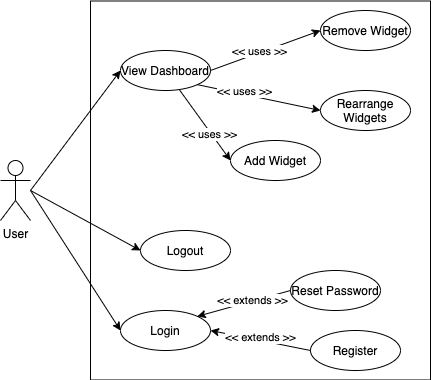
\includegraphics[width=0.6\textwidth]{Usecase.png}
		\end{center}
		\caption{Use Case Diagram}
		\label{fig:use case diagram}
	\end{figure}
	% End Section
	
	\section{Functional Requirements}
	\label{sec:functional_requirements}
	% Begin Section
	\begin{enumerate}[{VP}1]
		\item User
		\begin{enumerate}[{BE}1]
			\item User wants to view their \textit{dashboard}
			\begin{enumerate}
				\item The system will check if the user is logged in to their account with the system.
				\item If the user is not logged in, the system will redirect the user to the system registration page.
				\item The system will fetch the user's \textit{widgets} from the internal database.
				\item The system will display the user's  \textit{widgets} in accordance with the user's chosen positioning.
				\item The system will display the add and remove \textit{widget} options.
				\item The system will update the \textit{widgets} with current information.
				\item The users will be able to access more information by hovering over the associated help icons.
			\end{enumerate}
			\item User registers for an account
			\begin{enumerate}
				\item The system will provide the user with a sign up form.
				\item The system will verify the validity of the information and will create an account in the database if the information is valid.   
				\item The system will display an error message upon an invalid registration.
				\item The system will redirect the user to a newly created, empty \textit{dashboard} and will display system instructions.
			\end{enumerate}
			\item User attempts to login to the system
			\begin{enumerate}
				\item The system will display a login form.
				\item The system will verify that correct login information was provided.
				\item The system will redirect the user to their own \textit{dashboard}. 
				\item The system will display an error message after an invalid login attempt.
			\end{enumerate}
			\item User wants to add a \textit{widget} to their \textit{dashboard}
			\begin{enumerate}
				\item The system will provide the user with a list of possible \textit{widgets}. 
				\item The system will allow the user to input a \textit{widget} selection and will redirect them to the setup page for that \textit{widget}.
				\item After \textit{widget} configuration, the system will prompt the user to place the \textit{widget} on their \textit{dashboard}.
				\item The system will display an error message indicating any incorrect \textit{widget} parameters.
				\item The system will fetch the \textit{widget} data.
				\item The \textit{widget} and its parameters will be added to the system's database.
			\end{enumerate}
			\item User wants to remove a \textit{widget} from their \textit{dashboard}
			\begin{enumerate}
				\item The system will provide the user with a list of existing \textit{widgets} to delete. 
				\item The system will remove the selected \textit{widget} from the database.
				\item The system will remove the selected \textit{widget} from the \textit{dashboard}
			\end{enumerate}
			\item User wants to log out of the application
			\begin{enumerate}
				\item The system will invalidate the user's session.
				\item The user will be redirected to the login page.
			\end{enumerate}
			\item User wants to reset their password
			\begin{enumerate}
				\item The system will send a password reset email containing a temporary password.
				\item The user will be redirected to the change password page where they can modify their password.
			\end{enumerate}
			\item User wants to modify their \textit{dashboard} layout
			\begin{enumerate}
				\item The user will be able to reposition the widgets.
				\item The positioning of the \textit{widgets} will be updated in the system's database.
				\item The display will reflect the updated \textit{widget} positioning.
			\end{enumerate}
		\end{enumerate}
	\end{enumerate}
	
	% % End Section
	
	\section{Non-Functional Requirements}
	\label{sec:non-functional_requirements}
	% Begin Section
	\subsection{Look and Feel Requirements}
	\label{sub:look_and_feel_requirements}
	% Begin SubSection
	
	\subsubsection{Appearance Requirements}
	\label{ssub:appearance_requirements}
	% Begin SubSubSection
	\begin{enumerate}[{LF}1. ]
		\item The system shall use modern styling whenever possible.
		\item The system shall be visually appealing to 90\% of users.
	\end{enumerate}
	% End SubSubSection
	
	\subsubsection{Style Requirements}
	\label{ssub:style_requirements}
	% Begin SubSubSection
	\begin{enumerate}[{LF}1. ]
		\item The text size and font must be legible at a normal computer viewing distance of 20-40 inches \cite{OSHA}.
		\item The fonts, colours, and icons must remain consistent throughout the system.
	\end{enumerate}
	% End SubSubSection
	
	% End SubSection
	
	\subsection{Usability and Humanity Requirements}
	\label{sub:usability_and_humanity_requirements}
	% Begin SubSection
	
	\subsubsection{Ease of Use Requirements}
	\label{ssub:ease_of_use_requirements}
	% Begin SubSubSection
	\begin{enumerate}[{UH}1. ]
		\item Any buttons must be large enough to be located and pressed within 5 seconds.
		\item The users must be presented with general instructions when logging in for the first time.
		\item The language should be understandable to anyone with a fifth grade level of reading comprehension.
	\end{enumerate}
	% End SubSubSection
	
	\subsubsection{Personalization and Internationalization Requirements}
	\label{ssub:personalization_and_internationalization_requirements}
	% Begin SubSubSection
	\begin{enumerate}[{UH}1. ]
		\item Boardzilla must allow users to adjust the positioning and layering of the \textit{widgets} on their personal \textit{dashboard}.
		\item \textit{Widgets} must only accept valid parameters from users.
	\end{enumerate}
	% End SubSubSection
	
	\subsubsection{Learning Requirements}
	\label{ssub:learning_requirements}
	% Begin SubSubSection
	\begin{enumerate}[{UH}1. ]
		\item The user interface must be understood by a user within 10 minutes of system use.
	\end{enumerate}
	% End SubSubSection
	
	\subsubsection{Understandability and Politeness Requirements}
	\label{ssub:understandability_and_politeness_requirements}
	% Begin SubSubSection
	\begin{enumerate}[{UH}1. ]
		\item The symbols must convey the correct meaning to users 95\% of the time.
		\item The language in the app must be grammatically correct 99\% of the time.
	\end{enumerate}
	% End SubSubSection
	
	\subsubsection{Accessibility Requirements}
	\label{ssub:accessibility_requirements}
	% Begin SubSubSection
	\begin{enumerate}[{UH}1.]
		\item Any adjacent colours used within the user interface must appear distinct to users afflicted with colour blindness.
	\end{enumerate}
	% End SubSubSection
	
	% End SubSection
	\subsection{Performance Requirements}
	\label{sub:performance_requirements}
	% Begin SubSection
	
	\subsubsection{Speed and Latency Requirements}
	\label{ssub:speed_and_latency_requirements}
	% Begin SubSubSection
	\begin{enumerate}[{PR}1. ]
		\item The system shall respond to network requests with the necessary information in less than 3 seconds 99\% of the time.
		\item A request to fetch user data from the external \textit{APIs} must be sent in under 10 seconds 99\% of the time.
	\end{enumerate}
	% End SubSubSection
	
	\subsubsection{Safety-Critical Requirements}
	\label{ssub:safety_critical_requirements}
	% Begin SubSubSection
	\begin{enumerate}[{PR}1. ]
		\item \emph{N/A}
	\end{enumerate}
	% End SubSubSection
	
	\subsubsection{Precision or Accuracy Requirements}
	\label{ssub:precision_or_accuracy_requirements}
	% Begin SubSubSection
	\begin{enumerate}[{PR}1. ]
		\item The system must show correct \textit{widget} information 99\% of the time.
		\item The database must store current information 99.9\% of the time.
	\end{enumerate}
	% End SubSubSection
	
	\subsubsection{Reliability and Availability Requirements}
	\label{ssub:reliability_and_availability_requirements}
	% Begin SubSubSection
	\begin{enumerate}[{PR}1. ]
		\item Boardzilla shall be available for use 99.99\% of the time.
		\item The system shall require internet access to function.
	\end{enumerate}
	% End SubSubSection
	
	\subsubsection{Robustness or Fault-Tolerance Requirements}
	\label{ssub:robustness_or_fault_tolerance_requirements}
	% Begin SubSubSection
	\begin{enumerate}[{PR}1.]
		\item Boardzilla must display data consistently across supported devices.
		\item The system shall remain visible, but with stale data in the case of internet loss.
		\item The system shall notify active users in the case of a system failure, or loss of connectivity to the system.
	\end{enumerate}
	% End SubSubSection
	
	\subsubsection{Capacity Requirements}
	\label{ssub:capacity_requirements}
	% Begin SubSubSection
	\begin{enumerate}[{PR}1. ]
		\item The system shall be able to handle up to 100 users concurrently.
	\end{enumerate}
	% End SubSubSection
	
	\subsubsection{Scalability or Extensibility Requirements}
	\label{ssub:scalability_or_extensibility_requirements}
	% Begin SubSubSection
	\begin{enumerate}[{PR}1. ]
		\item The system shall be designed such that additional \textit{widgets} can be added in future versions without modifying more than 10\% of existing software.
	\end{enumerate}
	% End SubSubSection
	
	\subsubsection{Longevity Requirements}
	\label{ssub:longevity_requirements}
	% Begin SubSubSection
	\begin{enumerate}[{PR}1. ]
		\item The system shall remain online for at least 2 years after software delivery. 
	\end{enumerate}
	% End SubSubSection
	
	% End SubSection
	
	\subsection{Operational and Environmental Requirements}
	\label{sub:operational_and_environmental_requirements}
	% Begin SubSection
	
	\subsubsection{Expected Physical Environment}
	\label{ssub:expected_physical_environment}
	% Begin SubSubSection
	\begin{enumerate}[{OE}1. ]
		\item Boardzilla shall be operable in any physical environment that mobile phones or desktop computers can be operated in.
	\end{enumerate}
	% End SubSubSection
	
	\subsubsection{Requirements for Interfacing with Adjacent Systems}
	\label{ssub:requirements_for_interfacing_with_adjacent_systems}
	% Begin SubSubSection
	\begin{enumerate}[{OE}1. ]
		\item The application shall interface with \textit{APIs} that provide \textit{widget} data at no cost.
	\end{enumerate}
	% End SubSubSection
	
	\subsubsection{Productization Requirements}
	\label{ssub:productization_requirements}
	% Begin SubSubSection
	\begin{enumerate}[{OE}1. ]
		\item \emph{N/A}
	\end{enumerate}
	% End SubSubSection
	
	\subsubsection{Release Requirements}
	\label{ssub:release_requirements}
	% Begin SubSubSection
	\begin{enumerate}[{OE}1. ]
		\item The system must have 90\% of software issues patched before release.
	\end{enumerate}
	% End SubSubSection
	
	% End SubSection
	
	\subsection{Maintainability and Support Requirements}
	\label{sub:maintainability_and_support_requirements}
	% Begin SubSection
	
	\subsubsection{Maintenance Requirements}
	\label{ssub:maintenance_requirements}
	% Begin SubSubSection
	\begin{enumerate}[{MS}1. ]
		\item System updates shall not keep the system down for longer than 10 minutes.
		\item The system shall have an uptime of 99.99\%.
	\end{enumerate}
	% End SubSubSection
	
	\subsubsection{Supportability Requirements}
	\label{ssub:supportability_requirements}
	% Begin SubSubSection
	\begin{enumerate}[{MS}1. ]
		\item The system's instructions shall explain 99\% of application scenarios.
	\end{enumerate}
	% End SubSubSection
	
	\subsubsection{Adaptability Requirements}
	\label{ssub:adaptability_requirements}
	% Begin SubSubSection
	\begin{enumerate}[{MS}1. ]
		\item \emph{N/A}
	\end{enumerate}
	% End SubSubSection
	% End SubSection
	
	\subsection{Security Requirements}
	\label{sub:security_requirements}
	% Begin SubSection
	
	\subsubsection{Access Requirements}
	\label{ssub:access_requirements}
	% Begin SubSubSection
	\begin{enumerate}[{SR}1. ]
		\item The system shall only allow access if a valid username and password are entered.
		\item The system shall only provide a user with access to the \textit{dashboard} associated with their account.
	\end{enumerate}
	% End SubSubSection
	
	\subsubsection{Integrity Requirements}
	\label{ssub:integrity_requirements}
	% Begin SubSubSection
	\begin{enumerate}[{SR}1. ]
		% 	\item The system will not allow users to modify API's.
		\item The system must sanitize all data that is collected from users.
		\item The system must employ rate limiting to cap the addition of \textit{widgets} to one \textit{widget} per twenty seconds per user.
		\item The user must not be able to manipulate other user's data.
	\end{enumerate}
	% End SubSubSection
	
	\subsubsection{Privacy Requirements}
	\label{ssub:privacy_requirements}
	% Begin SubSubSection
	\begin{enumerate}[{SR}1. ]
		\item The system must not release user information to any third party.
		\item The system shall not store unencrypted user passwords.
		\item The system shall not collect any extraneous user data.
	\end{enumerate}
	% End SubSubSection
	
	\subsubsection{Audit Requirements}
	\label{ssub:audit_requirements}
	% Begin SubSubSection
	\begin{enumerate}[{SR}1. ]
		\item After a security audit, at least 90\% of the suggested changes should be made within a month.
	\end{enumerate}
	% End SubSubSection
	
	\subsubsection{Immunity Requirements}
	\label{ssub:immunity_requirements}
	% Begin SubSubSection
	\begin{enumerate}[{SR}1. ]
		\item Software security patches must be installed within a week of their release.
	\end{enumerate}
	% End SubSubSection
	
	% End SubSection
	
	\subsection{Cultural and Political Requirements}
	\label{sub:cultural_and_political_requirements}
	% Begin SubSection
	
	\subsubsection{Cultural Requirements}
	\label{ssub:cultural_requirements}
	% Begin SubSubSection
	\begin{enumerate}[{CP}1. ]
		\item The iconography and language contained within Boardzilla will be inoffensive to 99.9\% of users.
	\end{enumerate}
	% End SubSubSection
	
	\subsubsection{Political Requirements}
	\label{ssub:political_requirements}
	% Begin SubSubSection
	\begin{enumerate}[{CP}1. ]
		\item \emph{N/A}
	\end{enumerate}
	% End SubSubSection
	
	% End SubSection
	
	\subsection{Legal Requirements}
	\label{sub:legal_requirements}
	% Begin SubSection
	
	\subsubsection{Compliance Requirements}
	\label{ssub:compliance_requirements}
	% Begin SubSubSection
	\begin{enumerate}[{LR}1. ]
		\item The system must obey local laws and regulations.
		\item Boardzilla must follow the terms of service of all external \textit{APIs}.
	\end{enumerate}
	% End SubSubSection
	
	\subsubsection{Standards Requirements}
	\label{ssub:standards_requirements}
	% Begin SubSubSection
	\begin{enumerate}[{LR}1. ]
		\item \emph{N/A}
	\end{enumerate}
	% End SubSubSection
	
	% End SubSection
	
	% End Section
	\newpage
	\appendix
	\section{Division of Labour}
	\label{sec:division_of_labour}
	% Begin Section
	This document was created through a collaborative effort by the whole group, exchanging ideas and filling in sections together. Meetings were held regularly to iterate on this document until an acceptable final version was achieved. By signing this document, the group members certify that this division of labor is fair and accurate.
	
	\subsection{Signatures}
	\vspace{10ex}
	\begin{center}
		\noindent\begin{tabular}{ll}\\ 
			\makebox[3.5in]{\hrulefill} & \makebox[2in]	\hrulefill \\
			Matthew Paulin & Date\\[15ex]
			\makebox[3.5in]{\hrulefill} & \makebox[2in]	\hrulefill \\		
			Hargun Bedi & Date\\[15ex]
			\makebox[3.5in]{\hrulefill} & \makebox[2in]	\hrulefill \\		
			Dylan Smith & Date\\[15ex]
			\makebox[3.5in]{\hrulefill} & \makebox[2in]	\hrulefill \\		
			Chenwei Song & Date\\[15ex]
			\makebox[3.5in]{\hrulefill} & \makebox[2in]	\hrulefill \\
			Tianzheng Mai & Date\\
		\end{tabular}
	\end{center}
	% End Section
\end{document}
%------------------------------------------------------------------------------